\pdfpagewidth=8.5in
\pdfpageheight=11in
% The file ijcai21.sty is NOT the same than previous years'
\usepackage{ijcai21}

% Use the postscript times font!
\usepackage{times}
\usepackage{soul}
\usepackage{url}
\usepackage[hidelinks]{hyperref}
\usepackage[utf8]{inputenc}
\usepackage[small]{caption}
\usepackage{graphicx}
\usepackage{helvet}
\usepackage{amsthm}
\usepackage{booktabs}
\usepackage{algorithm}
\usepackage{algorithmic}
\urlstyle{same}
%
% PDF Info Is REQUIRED.
% For /Author, add all authors within the parentheses,
% separated by commas. No accents or commands.
% For /Title, add Title in Mixed Case.
% No accents or commands. Retain the parentheses.
\usepackage{amsmath}
\usepackage{amsthm}
\usepackage{booktabs}
\usepackage{algorithm}
\usepackage{algorithmic}
\usepackage{subcaption}
\usepackage[dvipsnames]{xcolor}
\usepackage{latexsym}
\newcommand{\ra}[1]{\renewcommand{\arraystretch}{#1}}
\newtheorem{theorem}{Theorem}
\newtheorem{proposition}{Proposition}
\newtheorem{conjecture}{Conjecture}
\newtheorem{definition}{Definition}
\newtheorem{lemma}{Lemma}
\def\tuple#1{( #1 )}




\begin{document}
\maketitle

\clearpage
\section*{Appendix}




\subsection*{Supplementary proofs}
In the appendix we use the term \emph{LB- (UB)-unsafe} to refer to a manipulation that lowers the lower (upper) bound of the manipulator. Also, recall that a \emph{solution} refers to any CS that satisfies the objective.

\subsection*{Proof of Theorem~\ref{thrm:egal_dir_add}}
Let 
$
u_0=\underset{P\in O(G)}{\min}(\{u(m,P)\}),
u_1=\underset{P\in O(G)}{\max}(\{u(m,P)\})
$.
We will refer to the CS yielding $u_0$ as $P_0$. Note that for every $P\in O(G)$ it holds that $Eg(P,G) \leq u_0 $
Assume by contradiction that Max-Egal is subject to UB-improvement.
That is, there exists a manipulation $r_{m}$ and a CS $P^m\in O(G^{m})$ such that $u(m,P^m) > u_1$. That is, $P^m\notin O(G)$.

Since the manipulator can only add edges it holds that $Eg(P^{m},G^m)\geq Eg(P_0,G)$. Moreover, if $Eg(P^{m},G^m)=Eg(P_0,G)$ then $P_{0}\in O(G^{m})$, which is not possible. Therefore, $Eg(P^{m},G^m)>Eg(P_0,G)$. Recall that in directed networks the utility of the other agents does not change. Therefore $\forall a \in A \setminus \{m\}$, \[
u(a,P^{m})  \geq Eg(P^{m},G^m) > Eg(P_0,G).
\]
In addition, $u(m,P^{m})>u_1\geq Eg(P_0,G)$. 
Overall, $\forall a \in A, u(a,P^{m}) \geq Eg(P_0,G)$. That is, $Eg(P^{m},G) \geq Eg(P_0,G)$, and thus $P^m\in O(G)$, which is a contradiction.


Now, assume by contradiction that Max-Egal is subject to LB-improvement.
That is, there exists a manipulation $r_{m}$ such that
\begin{equation} \label{ineq:egal_dir}
\forall \  P \in O(G^m), u(m,P) > u_0.
\end{equation} That is $P_0\notin O(G^m)$.
Denote an arbitrary CS in $O(G^m)$ as $P^m$. 
It holds that $Eg(P^m,G^m)>Eg(P_0,G^m)$ and $Eg(P_0,G)\geq E(P^m,G)$.

Again, in directed networks the utility of the other agents does not change. Therefore if after the manipulation $Eg(P^m,G^m)>Eg(P^m,G)$ it can only change by the utility of $m$. But $u(a,P^m)>u(a,P)$, hence even before the manipulation $Eg(P^m,G^m)>Eg(P^m,G)$, in contradiction.



\subsection*{Proof of Theorem~\ref{thm:all_distance1}}

\subsubsection*{Max-Util}
If $0<|N(m)|<n-1$, by looking at possible networks like the ones in Figures \ref{fig:distance1_util_unsafe_add_LB},\ref{fig:distance1_util_unsafe_add_UB} we can see that adding any edge is LB- and UB-unsafe respectively.
These examples can be tweaked to fit any number of agents and any number of desired agents the manipulator has.
If $|N(m)|=n-1$ the manipulator cannot add edges.


\subsubsection*{Max-Egal}
Obviously adding or removing in undirected networks is both LB- and UB-unsafe. Adding an edge towards agent $a_0$ can lead to utility $0$ when the maximum egalitarian SW is $1$, if $m$ ends up in a coalition alone with $a_0$.
Removing an edge can lead to utility $0$. If one $m$'s neighbours has no other agents, removing that edge results in maximum egalitarian SW $0$, hence the lower bound is also $0$. So both add and remove are LB-unsafe.
For the cases of $|N(m)|<n-3, |N(m)|=n-2$ and $|N(m)|=n-1$ see Figures~\ref{fig:egalremove1},\ref{fig:egalremove2} and \ref{fig:egalremove3} for proofs that removing is UB-unsafe, respectively. If $m$ has more neighbours can just add nodes on the top, and more non-neighbours in bottom of the figures.
Figure~\ref{fig:egalremove4} provides proof that adding UB-unsafe. For higher numbers both neighbours and non-neighbours are added at the bottom. Note that this example requires at least neighbours ($|N(m)|\geq2$. However, if $m$ has only one neighbour it is easy to see no manipulation is beneficial against Max-Egal.


\subsubsection*{At-Least-1}
Adding any edge to another agent $a_0$ might result in a LB- of $0$. That is because the CS where $a_0$ and $m$ form one coalition could be a solution now.
Any partial network in distance 1 can have a possible network with a solution where $m$'s original LB- is higher than $0$, hence adding is LB-unsafe.

% In the case with the equal size constraint, the same could be said. However, in this scenario the difference would be that $m$'s LB is not necessarily $0$. If $|N(m)| < n/2$, it could be lower to $0$.
% If $n/2 \leq |N(m)|$ neighbours, there is a possible network where $m$ is guaranteed utility of $n/2 -1 $. Therefore, adding the edge comes at the cost of a true friend, lowering the LB to $n/2-2$.


For At-Least-1, all that is left to prove is that against manipulator $m^-$ the objective is LB-proof. Of course, over undirected networks it is true, as any removal might lead to an infeasible instance.

Over directed networks, it is also easy to see the any removal may lead to an infeasible instance; If $m$ has at least one neighbour $a_0$ for which both $(a_0,m),(m,a_0)\in E $, it could be the case that the only solution is where $m$ and $a_0$ form a coalition alone. (If all of the other agents form a directed circle, and have no other edges but ones going to or from $m$). In that case removing is LB-unsafe.
If $m$ does not have a neighbour like that, the same example still applies when the only solution is $m$ alongside one of his out-neighbours and another agent. i.e. $a_0,a_1$ where $(m,a_0),(a_0,a_1),(a_1,a_0)\in E$.


\clearpage
\subsection*{Equal Size}
An important constraint that arises in many real world scenarios is that all of the coalitions should be of the same size. For example, when dividing students into classes it is common to ask that all of the classes consist of roughly the same number of students.
Therefore we also consider the setting in which all of the coalitions are of the size $n/k$, if $n/k$ is an integer. Otherwise, some coalitions are of size $\left \lceil{n/k}\right \rceil$ and some are of size $\left \lfloor{n/k}\right \rfloor$. We call this restriction the Equal Size constraint, and through the paper we analyze the different objectives with or without it.

Due to space constraints, the definition and results of the equal size constraints have been moved to the appendix. All of the resistance results from Section~\ref{sec:full_info} still stand with the equal size constraint. The susceptibility results are summarized in Table~\ref{tbl:distnce2_equalsize}.




\begin{table}[htp]

\ra{1}
\begin{tabular}{@{}lcccr@{}}\toprule 
$Objective$ & $M$ & $Network$ & $Type$ & $Figure$\\\midrule
Max-Util & A & Both & Strict & \ref{fig:util_size_add}\\
Max-Util & R & Both & Strict & \ref{fig:Util_size_remove}\\
Max-Egal & A & Undirected & LB & \ref{fig:Egal_size_undirected_add_LB}\\
Max-Egal & A & Undirected & UB & \ref{fig:Egal_size_undirected_add_UB}\\
At-Least-1 & A & Undirected & Strict & \ref{fig:Least1_size_undirected_add}\\
At-Least-1 & R & Both & LB & \ref{fig:least1_size_remove}\\
\bottomrule
\end{tabular}
\caption{Summary of susceptibility results for distance 2 with the equal size constraint.
Key: A = add, R = Remove, LB/UB/Strict = the objective is subject to LB/UB/Strict-improvement.
}
\label{tbl:distnce2_equalsize}
\end{table}

\begin{proposition}
\label{thm:util_distance1}
Max-Util with the equal size constraint is subject to 1-safe LB- and UB-improvement and is 1-safe weak-proof for a manipulator $m^-$ over directed and undirected networks. 
\end{proposition}

\begin{proof}
See Figures~\ref{fig:distance1_util/egal_lb} and \ref{fig:distance1_util_ub} for the 1-safe LB-improvement and 1-safe UB-improvement, respectively. We move on to prove it is 1-safe weak-proof.

First, we prove that if the manipulator has less than $n-1$ neighbours, no UB-safe manipulation exists.
If $0<|N(m)|\leq \lfloor n/2 \rfloor$ then Figures~\ref{fig:thrm5_1} and \ref{fig:thrm5_2} provide examples for UB-unsafe scenarios for even and odd $n$, respectively.
If $\lfloor n/2 \rfloor<|N(m)| < n/2$ then Figures~\ref{fig:thrm5_3} and \ref{fig:thrm5_4} provide examples for UB-unsafe scenarios for even and odd $n$, respectively.

If $|N(m)| = n-1$, then if $n$ is even, the manipulator always gets the same utility and no manipulation is possible.
If $n$ is odd we have shown it is subject to LB and UB 1-safe improvement.
If the manipulator removes more than 1 edge, Figure~\ref{fig:thrm5_5} provides an example that this is UB-unsafe.

By removing only 1 edge, the manipulation cannot be weak-improvement. 
Denote the utilitarian SW of coalition structure $P$ in $G$ as $Ut(P,G)$.
Let 
$
u_0=\underset{P\in O(G)}{\min}(\{u(m,P)\}),
u_1=\underset{P\in O(G)}{\max}(\{u(m,P)\})
$.
We will refer to the CS yielding $u_0$ as $P_0$.
Assume by contradiction that Max-Util is subject to weak-improvement when removing only 1 edge.
That is, there exists a manipulation $r_{m}$ and a CS $P^m\in O(G^{m})$ such that $u(m,P^m) > u_1$. That is, $P^m\notin O(G)$. Also, $P_0\notin O(G^m)$.

Therefore, we can see that $Ut(P_0,G) > Ut(P^m,G)$ and $Ut(P^m,G^m)>Ut(P_0,G^m)$.
Since the manipulator is only able to remove edges it holds that $Ut(P^m,G^m)\leq Ut(P^m,G)$. So we get that $Ut(P_0,G) > Ut(P^m,G^m) \xrightarrow{} Ut(P_0,G) - 1 \geq Ut(P^m,G^m)$
Since only 1 edge was removed, the utilitarian SW could drop at most by $1$ and it holds that $Ut(P^0,G) - 1 \leq Ut(P^0,G^m)$.
Combining the last two inequalities we get $ Ut(P_0,G^m) \geq Ut(P_m,G^m) $ in contradiction.
\end{proof}


\begin{proposition}
\label{thm:Egal_distance1}
Max-Egal with the equal size constraint is subject to 1-safe LB-improvement and is 1-safe UB-proof for a manipulator $m^-$ over directed networks.
\end{proposition}

\begin{proof}
See Figure~\ref{fig:distance1_util/egal_lb} for the 1-safe LB-improvement.

For the cases of $|N(m)|<n-3, |N(m)|=n-2$ and $|N(m)|=n-1$ Figures~\ref{fig:egalremove1},\ref{fig:egalremove2} and \ref{fig:egalremove3} show the that removing any edge is UB-unsafe, respectively.
\end{proof}

\begin{proposition}
\label{thm:least1_distance1_es}
At-Least-1 with the equal size constraint is subject to 1-safe UB-improvement and is 1-safe LB-proof for a manipulator $m^+$ over undirected networks.
\end{proposition}

\begin{proof}
See Figure~\ref{fig:distance1_least1} for the 1-safe UB-improvement.
The resistance proof is the same as without the equal size constraint.
\end{proof}


\begin{theorem}
\label{thm:all_distance1_es}
Except for the situations in Theorems~\ref{thm:util_distance1},\ref{thm:Egal_distance1} and \ref{thm:least1_distance1_es}, all of our objectives with the equal size constraint are 1-safe strategyproof. 
\end{theorem}
Here we separate the proof between the objectives as well:
\subsubsection*{Max-Util}
To show the manipulation is LB-unsafe;
If $0<|N(m)|\leq \lfloor n/2 \rfloor$ then Figures~\ref{fig:unsafeutil3} and \ref{fig:unsafeutil4} provide examples for even and odd $n$, respectively.
If $\lfloor n/2 \rfloor<|N(m)| < n/2$ then Figures~\ref{fig:unsafeutil7} and \ref{fig:unsafeutil8} provide examples for even and odd $n$, respectively.

To show the manipulation is UB-unsafe;
If $0<|N(m)|\leq \lfloor n/2 \rfloor$ then Figures~\ref{fig:unsafeutil1} and \ref{fig:unsafeutil2} provide examples for even and odd $n$, respectively.
If $\lfloor n/2 \rfloor<|N(m)| < n/2$ then Figures~\ref{fig:unsafeutil5} and \ref{fig:unsafeutil6} provide examples for even and odd $n$, respectively.


\subsubsection*{Max-Egal}
Manipulator $m^-$:
If $|N(m)| \leq n/2 -1$, a possible network which is an $n-1$ clique except for $m$ yields an egalitarian SW of exactly $|N(m)|$. Removing any of her neighbours is LB-unsafe as she is guaranteed to get all of the neighbours she reports.
Now look at a possible network where $|N(m)|-1$ neighbours of $m$ are connected only to her and all non-neighbours of $m$ are connected to another node $a_0$. Out of the non-neighbours, $n/2 -2 $ nodes have no more edges. The others are neighbours to neighbours of $m$. The last neighbour of $m$ is connected also to $a_0$. Of course, the maximum possible egalitarian SW is $1$, and the two possible outcomes for $m$ are either getting all the neighbours, or not getting the single neighbours which is connected to $a_0$. By removing an edge it might be the case that this single neighbour is the one being disconnected, hence removing an edge is UB-unsafe.
If $n/2 -1 < |N(m) < n-1$, look at a possible network where $n/2-1$ of neighbours of $m$ form a path $a_1, a_2, .. ,a_{n/2-1}$. All the other nodes form a clique of size $n/2$ and one of them $a_0$ is connected to $a_1$. The highest egalitarian SW achievable is $2$, by putting $m$ alongside the path. By removing the edge towards $a_1$ or $a_2$ the highest egalitarian SW possible is now 1, and it can also be achieved by swapping $m$ and $a_0$. Hence removing is LB-unsafe.
In a possible network where the $n/2-1$ neighbours are connected only to $m$ and $a_0$ (but not between themselves) the highest egalitarian SW possible is $1$, either by $m$ or $a_0$ being with the $n/2-1$ neighbours. By removing an edge towards one of the neighbours, $m$ is guaranteed to not be with them, but in the other coalition with only one neighbour, hence removing is UB-unsafe.
If $|N(m)=n-1$, if $n$ is even no manipulation is beneficial as the manipulator always gets her highest utility. 
If $n$ is odd, the possible network could be made of two cliques $L_1$ and $L_2$ of sizes $n-1/2$ and $n-1/2 -1$, and $L_1$ is missing 1 edge between two nodes $a_1, a_2$. The last node $a_0$ is connected to the whole network just like $m$. The two possible CSs yielding an egalitarian SW of $n-1/2 -1$ are where $L_1$ form a coalition alongside either $m$ or $a_0$ and $L_2$ is with the other. Hence the upper bound for $m$ is $n-1/2$. By removing an edge towards either $a_1$ or $a_2$, $m$ is guaranteed to be with $L_2$, so removing is UB-unsafe.

Manipulator $m^+$:
If $|N(m)| \leq n/2 -1 $, look at a network that is made of a star of size $n/2$ that includes all of $m$'s neighbour, another star of size $n/2-2$, and a node $a_0$ with no edges. Adding an edge towards $a_0$ is guaranteeing utility $0$ for the manipulator, as him being  being with $a_0$ and the smaller star is the only CS yielding egalitarian SW of $1$. Hence it is both LB and UB-unsafe.
If $n/2-1 < |N(m)| < n-1$, it is possible the graph is a clique guaranteeing $m$ a full coalition of neighbours. By adding any edge this might make some of the neighbours fake, therefore UB-unsafe. Lastly, look at a graph where $n/2 -1$ neighbours of $m$ form a circle $C_m$. Also, another $n/2-1$ nodes form a circle $C_0$, and call the last node $a_0$. $a_0$ is connected to two nodes $C_0$ and to one in $C_m$. Also, there is a node $a_1$ in $C_m$ that is connected to two nodes in $C_0$. Adding an edge to $a_0$ is LB-unsafe, as now a CS where $m$ is with $a_0$ instead of $a_1$ is a solution.

\subsubsection*{At-Leas-1}
If $|N(m)|<\lfloor n/2 \rfloor$, removing can still lead to an infeasible instance. If $|N(m)|<\lfloor n/2 \rfloor$ then removing edges while still having more than $\lfloor n/2 \rfloor$ does not change the outcome, as any previous solution is still satisfying At-Least-1. This is because the manipulator is still guaranteed at least $1$ out neighbour in every CS, and the other agents' utility has not changed. Removing edge until having less than $\lfloor n/2 \rfloor$ can again result in infeasible instance.

\begin{figure*}[t]
    \centering
    \begin{subfigure}{0.6\textwidth}
    \centering  
        \begin{subfigure}{0.15\textwidth}
        \renewcommand\thesubfigure{\alph{subfigure}1}
            \centering
        \includegraphics[page=5,width=\textwidth]{Graphs/graphs.pdf}
        \caption{\\U/S/ES}
        \label{fig:util_size_add}
        \end{subfigure}
        \hfill
        \begin{subfigure}{0.15\textwidth}
            \addtocounter{subfigure}{-1}
            \renewcommand\thesubfigure{\alph{subfigure}2}
            \centering
        \includegraphics[page=23,width=\textwidth]{Graphs/graphs.pdf}
        \caption{\\E/LB/ES}
        \label{fig:Egal_size_undirected_add_LB}
        \end{subfigure}
        \hfill
        \begin{subfigure}{0.15\textwidth}
            \addtocounter{subfigure}{-1}
            \renewcommand\thesubfigure{\alph{subfigure}3}
            \centering
        \includegraphics[page=25,width=\textwidth]{Graphs/graphs.pdf}
        \caption{\\E/UB/ES}
        \label{fig:Egal_size_undirected_add_UB}
        \end{subfigure}
        \hfill
        \begin{subfigure}{0.15\textwidth}
                    \addtocounter{subfigure}{-1}
            \renewcommand\thesubfigure{\alph{subfigure}4}
            \centering
        \includegraphics[page=33,width=\textwidth]{Graphs/graphs.pdf}
        \caption{\\1/S/ES}
        \label{fig:Least1_size_undirected_add}
        \end{subfigure}
    \addtocounter{subfigure}{-1}
    \caption{$m^+$}
    \label{fig:add_es_subfig} 
    \end{subfigure}
    \hfill
    \begin{subfigure}{0.3\textwidth}
    \centering  
        \begin{subfigure}{0.3\textwidth}
            \renewcommand\thesubfigure{\alph{subfigure}1}
            \centering
        \includegraphics[page=45,width=\textwidth]{Graphs/graphs.pdf}
        \caption{\\U/S/ES}
        \label{fig:Util_size_remove}
        \end{subfigure}    
        \hfill
        \begin{subfigure}{0.3\textwidth}
        \addtocounter{subfigure}{-1}
        \renewcommand\thesubfigure{\alph{subfigure}2}
            \centering
        \includegraphics[page=21,width=\textwidth]{Graphs/graphs.pdf}
        \caption{\\E/S/ES}
        \label{fig:Egal_size_remove}
        \end{subfigure}
        \hfill
        \begin{subfigure}{0.3\textwidth}
                    \addtocounter{subfigure}{-1}
        \renewcommand\thesubfigure{\alph{subfigure}3}
        \centering
        \includegraphics[page=27,width=\textwidth]{Graphs/graphs.pdf}
        \caption{\\1/LB/ES}
        \label{fig:least1_size_remove}
        \end{subfigure}    
        \addtocounter{subfigure}{-1}
    \caption{$m^-$}
    \label{fig:remove_es_subfig} 
    \end{subfigure}
%    \hfill
%    \begin{subfigure}{0.1\textwidth}

%        \renewcommand\thesubfigure{\alph{subfigure}1}
%    \centering
%        \begin{subfigure}{0.4\textwidth}
%        \centering
%        \includegraphics[page=9,width=\textwidth]{Graphs/Distance 1 manipulation.pdf}
%        \caption{\\E/UB}
%        \label{fig:distance1_egal_ub_any}
%    \end{subfigure} \hfill
%        \begin{subfigure}{0.4\textwidth}
%        \addtocounter{subfigure}{-1}
%        \renewcommand\thesubfigure{\alph{subfigure}2}
%        \centering
%        \includegraphics[page=7,width=\textwidth]{Graphs/Distance 1 manipulation.pdf}
%        \caption{\\1/UB}
%        \label{fig:distance1_least1}
%    \end{subfigure}
%    \addtocounter{subfigure}{-1}
%    \caption{Distance 1}
    %%graphs showing manipulation of different objectives by adding edges. Dotted edges are added by the manipulator.
%    \label{fig:distance1_manipulation}
%    \end{subfigure}
    
    
    \caption{Figures providing examples of susceptibility to manipulation with the equal size constraint. Key: U=Max-Util, E=Max-Egal, 1=At-least-1, S=strict-improvement, UB=UB-improvement, LB=LB-improvement}
    %graphs showing manipulation of different objectives by adding edges. Dotted edges are added by the manipulator.
    \label{fig:es_graphs}
\end{figure*}

\begin{figure}
    \centering
    \begin{subfigure}{0.07\textwidth}
        \centering
        \includegraphics[page=1,width=\textwidth]{Graphs/Distance 1 special cases.pdf}
        \caption{R,UB}
        \label{fig:thrm5_1}
    \end{subfigure}
    \hfill
    \begin{subfigure}{0.07\textwidth}
        \centering
        \includegraphics[page=2,width=\textwidth]{Graphs/Distance 1 special cases.pdf}
        \caption{R,UB}
        \label{fig:thrm5_2}
    \end{subfigure}
    \hfill
    \begin{subfigure}{0.07\textwidth}
        \centering
        \includegraphics[page=3,width=\textwidth]{Graphs/Distance 1 special cases.pdf}
        \caption{R,UB}
        \label{fig:thrm5_3}
    \end{subfigure}
    \hfill
    \begin{subfigure}{0.07\textwidth}
        \centering
        \includegraphics[page=4,width=\textwidth]{Graphs/Distance 1 special cases.pdf}
        \caption{R,UB}
        \label{fig:thrm5_4}
    \end{subfigure}
    \hfill
    \begin{subfigure}{0.07\textwidth}
        \centering
        \includegraphics[page=5,width=\textwidth]{Graphs/Distance 1 special cases.pdf}
        \caption{R,UB}
        \label{fig:thrm5_5}
    \end{subfigure}
    \\
    \begin{subfigure}{0.07\textwidth}
        \centering
        \includegraphics[page=6,width=\textwidth]{Graphs/Distance 1 special cases.pdf}
        \caption{A,UB}
        \label{fig:unsafeutil1}
    \end{subfigure}
    \hfill
    \begin{subfigure}{0.07\textwidth}
        \centering
        \includegraphics[page=7,width=\textwidth]{Graphs/Distance 1 special cases.pdf}
        \caption{A,UB}
        \label{fig:unsafeutil2}
    \end{subfigure}
    \hfill
    \begin{subfigure}{0.07\textwidth}
        \centering
        \includegraphics[page=8,width=\textwidth]{Graphs/Distance 1 special cases.pdf}
        \caption{A,LB}
        \label{fig:unsafeutil3}
    \end{subfigure}
    \hfill
    \begin{subfigure}{0.07\textwidth}
        \centering
        \includegraphics[page=9,width=\textwidth]{Graphs/Distance 1 special cases.pdf}
        \caption{A,LB}
        \label{fig:unsafeutil4}
    \end{subfigure}
    \\
    \begin{subfigure}{0.07\textwidth}
        \centering
        \includegraphics[page=10,width=\textwidth]{Graphs/Distance 1 special cases.pdf}
        \caption{A,UB}
        \label{fig:unsafeutil5}
    \end{subfigure}
    \hfill
    \begin{subfigure}{0.07\textwidth}
        \centering
        \includegraphics[page=11,width=\textwidth]{Graphs/Distance 1 special cases.pdf}
        \caption{A,UB}
        \label{fig:unsafeutil6}
    \end{subfigure}
    \hfill
    \begin{subfigure}{0.07\textwidth}
        \centering
        \includegraphics[page=12,width=\textwidth]{Graphs/Distance 1 special cases.pdf}
        \caption{A,LB}
        \label{fig:unsafeutil7}
    \end{subfigure}
    \hfill
    \begin{subfigure}{0.07\textwidth}
        \centering
        \includegraphics[page=13,width=\textwidth]{Graphs/Distance 1 special cases.pdf}
        \caption{A,LB}
        \label{fig:unsafeutil8}
    \end{subfigure}
    \caption{Unsafe manipulations, Max-Util, with the equal size constraint. Legend: A - add, R - remove, LB/UB - LB/UB-unsafe. In the figures $n$ stands for the total number of agents and $x$ for any number between $0$ and the clique's size}
    %graphs showing manipulation of different objectives by adding edges. Dotted edges are added by the manipulator.
    \label{fig:unsafe_util_equalsize}
\end{figure}


\begin{figure}
    \centering
\begin{subfigure}{0.07\textwidth}
        \centering
        \includegraphics[page=1,width=\textwidth]{Graphs/Distance 1 util unsafe.pdf}
        \caption{R/LB}
        \label{fig:distance1_util_unsafe_remove_LB_appendix}
    \end{subfigure}
    \hfill
    \begin{subfigure}{0.07\textwidth}
        \centering
        \includegraphics[page=2,width=\textwidth]{Graphs/Distance 1 util unsafe.pdf}
        \caption{R/UB}
        \label{fig:distance1_util_unsafe_remove_UB_appendix}
    \end{subfigure}
    \hfill
    \begin{subfigure}{0.07\textwidth}
        \centering
        \includegraphics[page=3,width=\textwidth]{Graphs/Distance 1 util unsafe.pdf}
        \caption{A/LB}
        \label{fig:distance1_util_unsafe_add_LB}
    \end{subfigure}
    \hfill
    \begin{subfigure}{0.07\textwidth}
        \centering
        \includegraphics[page=4,width=\textwidth]{Graphs/Distance 1 util unsafe.pdf}
        \caption{A/UB}
        \label{fig:distance1_util_unsafe_add_UB}
    \end{subfigure}

    \caption{Unsafe manipulations, Max-Util. Legend: A - add, R - remove, LB/UB - LB/UB-unsafe}
    %graphs showing manipulation of different objectives by adding edges. Dotted edges are added by the manipulator.
    \label{fig:distance1_unsafe_util_appendix}
\end{figure}

\begin{figure}
    \centering
    \begin{subfigure}{0.07\textwidth}
        \centering
        \includegraphics[page=1,width=\textwidth]{Graphs/egal unsafe distance1.pdf}
        \caption{R/UB}
        \label{fig:egalremove1}
    \end{subfigure}
    \hfill
    \begin{subfigure}{0.07\textwidth}
        \centering
        \includegraphics[page=2,width=\textwidth]{Graphs/egal unsafe distance1.pdf}
        \caption{R/UB}
        \label{fig:egalremove2}
    \end{subfigure}
    \hfill
    \begin{subfigure}{0.07\textwidth}
        \centering
        \includegraphics[page=3,width=\textwidth]{Graphs/egal unsafe distance1.pdf}
        \caption{R/UB}
        \label{fig:egalremove3}
    \end{subfigure}
    \hfill
    \begin{subfigure}{0.07\textwidth}
        \centering
        \includegraphics[page=4,width=\textwidth]{Graphs/egal unsafe distance1.pdf}
        \caption{A/UB}
        \label{fig:egalremove4}
    \end{subfigure}

    \caption{Unsafe manipulations, Max-Egal. Legend: A - add, R - remove, LB/UB - LB/UB-unsafe}
    %graphs showing manipulation of different objectives by adding edges. Dotted edges are added by the manipulator.
    \label{fig:distance1_unsafe_egal}
\end{figure}

\begin{figure}
    \centering
    \begin{subfigure}{0.07\textwidth}
        \centering
        \includegraphics[page=2,width=\textwidth]{Graphs/Distance 1 manipulation.pdf}
        \caption{\\U,E/LB}
        \label{fig:distance1_util/egal_lb}
    \end{subfigure} \hspace{20pt}
    \begin{subfigure}{0.07\textwidth}
        \centering
        \includegraphics[page=4,width=\textwidth]{Graphs/Distance 1 manipulation.pdf}
        \caption{\\U/UB}
        \label{fig:distance1_util_ub}
    \end{subfigure} \hspace{20pt}
    \begin{subfigure}{0.07\textwidth}
        \centering
        \includegraphics[page=7,width=\textwidth]{Graphs/Distance 1 manipulation.pdf}
        \caption{\\1/UB}
        \label{fig:distance1_least1}
    \end{subfigure}
    \caption{Manipulations by removing edges, for distance 1. Legend: Objective/Manipulation~Type. Key: U=Max-Util, E=Max-Egal, 1=At-Least-1, UB=UB-improvement, LB=LB-improvement.}
    %graphs showing manipulation of different objectives by adding edges. Dotted edges are added by the manipulator.
    \label{fig:distance1_manipulation}
\end{figure}


\clearpage

\subsection*{Max-Util Distance 2 Conjecture}
\begin{conjecture}
\label{conj:util}
Max-Util is 2-safe weak-proof against manipulator $m^-$ over undirected networks.
\end{conjecture}

We lay out some of the advances we have made trying to prove the conjecture:

Let $G_2=(A,E)$ be a partial network and $m^-$ a manipulator. Assume by negation a 2-safe weak-improvement $r^m$ exists over $G_2$. Hence there exists a possible game $\overline{G}$ of $G_2$ for which $r^m$ is a weak-improvement. We want to show that either the manipulation does not really improve the upper bound, or there exists another supplement $\overline{G'}$ of $G$ for which $r^m$ lowers the manipulator's upper bound.

Denote $\overline{G}^m$ as the network $\overline{G}$ after the manipulation $r^m$. Let $P^m=\{B_1,B_2\}$ be (one of) the CSs with higher utility for $m$ than all CSs in $\overline{G}$, and denote by $B_1$ the coalition in which $m$ is. Formally:
\begin{equation}
\label{ineq:util_ub_safe}
u(m,P_m) > \underset{P\in O_{obj}(\overline{G})}{\min}(u(m,P)).    
\end{equation}
Denote by $c_0$ and $c_m$ the minimum cut size of $\overline{G}$ and $\overline{G}^m$ respectively.
We will define $c(P,G)$ as the cut size of coalition structure $P$ in network $G$.


\begin{lemma}
$B_2$ contains at least $2$ node $a_1,a_2$ such that $a_1,a_2\in N$ and $a_1,a_2\notin N^m$.
\end{lemma}
\begin{proof}
Since $r^m$ is a LB-improvement there is a solution for $\overline{G}$ which is not a solution in $\overline{G}^m$. Since we only removed edges, the only reason it would happen is that $c_0 > c_m$.
Since $P^m$ is not a solution in $\overline{G}$ (as it is better than all solutions in it) we get that $c(P^m,\overline{G}) > c_0$. Combining both outcomes we get that $c(P^m,\overline{G}) \geq c_m+2$. Because we know that $c(P^m,\overline{G}^m) = c_m$ and the only changes between $\overline{G}$ and $\overline{G}^m$ are edges that the manipulator removed, it has to be the case that he removed at least $2$ edges going out to $B_2$.
\end{proof}
We get that the maximum utility $m$ can have after the manipulation is $|N(m)|-2$. Because of that, the minimum degree $\delta(\overline{G}) = min(\{deg(v) | v\in V\ and v != m \})$ of all the nodes but $m$ is at least $c_0+1$. Otherwise the CS where a node with at most $c_0$ neighbours is alone is a minimal cut and yields $m$ a utility of $|N(m)|-1$ or $|N(m)|$ in contradiction to inequality~\ref{ineq:util_ub_safe}.

We distinguish between multiple cases. 
Case one: $B_2\subseteq N$, i.e. contains only true neighbours of $m$.
Since $P^m$ has higher utility for the manipulator than all previous solutions, in all previous solutions there are at least $|B_2|+1$ neighbours of her not in her coalition. Hence $c_0 \geq |B_2|+1$. By the previous statement we get that $\delta(\overline{G}) \geq |B_2| + 2$. Since the manipulator might have removed one edge in $\overline{G}^m$ , we get that $\delta(\overline{G}^m) \geq |B_2| + 1$. Because of that, in $P^m$ every node in $B_2$ has at least $2$ neighbours outside $B_2$, which we concludes that $c_m \geq 2|B_2| \rightarrow c_0 > 2|B_2| \rightarrow \delta(\overline{G}) > 2|B_2| + 1 \rightarrow \delta(\overline{G}^m) \geq 2|B_2|+1$. Hence all nodes in $B_2$ has at least $|B_2|+2$ edges going out from $B_2$, so we get that $c_m > |B_2|*(|B_2|+2)$. By repeating this process we get that the cut is unbounded, in contradiction since the network is finite.

Case two: $|B_2\cap N| = |B_2| -1$, i.e. $B_2$ contains exactly one non-neighbour of $m$, denote her by $a$.
By the same logic from above we get that $c_0 \geq |B_2|$ (as in $P^m$ the manipulator only has $|B_2| -1$ neighbours. So $\delta(\overline{G}) \geq |B_2| + 1 \rightarrow \delta(\overline{G}^m) \geq |B_2|$. Since $a$ is not a neighbour of $m$, her degree in $\overline{G}^m$ has not changed and it is still at least $|B_2| +1$. In conclusion in $B_2$ we have $|B_2|-1$ nodes of degree at least $|B_2|$ and one with at least $|B_2| +1$. Hence $c_m \geq |B_2| +1 \rightarrow c_0 \geq |B_2| + 2$, and yet again by repeating the process we get that the cut is unbounded.

Case three: $B_2$ contains at least 2 non-neighbours of $m$.

This is the case we could not prove. Note that in any solution in Max-Util any agent is guaranteed to be in the coalition where she has more neighbours. Therefore if $B_2$ contains at least $2$ neighbours of $m$, then $B_1$ contains at least $3$. However, if the manipulator had only $5$ neighbours originally, he would have had at least $3$ neighbours before the manipulation. So he has at least $4$ neighbours in $B_1$.


To sum it up, if a weak-improvement did exist, it has to be that $B_1$ contains at least $4$ neighbours of $m$, $B_2$ contains at least $2$ neighbours and $2$ non-neighbours of $m$, and the minimum degree of the graph is at least $4$.



\end{document}